\chapter{Questões de Pesquisa}
\label{cap:qp}

Este trabalho propõe um estudo sobre as \textit{breaking changes} em \textit{releases minor} e \textit{patch} e seus impactos no ecossistema do \textsf{npm}. Para isso, três questões de pesquisa foram desenvolvidas para que seja possível executar o estudo. A seguir, há a motivação para cada questão de pesquisa. Nesta Seção estão descritos os métodos utilizados para responder cada uma das questões de pesquisa.

%---------------------------------------------------%
%----------------------RQ1--------------------------%
%---------------------------------------------------%

\section{QP1. Com que frequência \textit{breaking changes} impactam os clientes?}
\label{sec:qp1}

\subsubsection{Motivação}
\label{sec:qp1:motivation}
No ecossistema do \textsf{npm}, uma \textit{release} que contenha um erro pode afetar uma grande quantidade de pacotes, uma vez que a rede de dependências do \textsf{npm} é relativamente densa \cite{teorical_reference:npm_2}. Para evitar que \textit{breaking changes} se manifestem nos clientes, os provedores introduzem as \textit{breaking changes} em \textit{releases major}, seguindo o padrão do Versionamento Semântico, e os clientes podem utilizar \textit{strings semver} para aceitar apenas as versões \textit{minor} e \textit{patch} dos provedores -- o que é o padrão do \textsf{npm}. Entretanto, nem sempre o provedor é capaz de distinguir se suas alterações são ou não \textit{breaking changes} \cite{noregrets2018}, ou, muitas vezes, as \textit{breaking changes} são introduzidas sem que os provedores percebam. Estudos anteriores têm estudado \textit{breaking changes} no ecossistema do \textsf{npm} \cite{using_others_tests, noregrets2018, intro:break_change, teorical_reference:bc_1}, mas não estudaram a frequência e como se manifestam. Nesta RQ, serão quantificadas as manifestações das \textit{breaking changes} nos clientes.

\subsubsection{Método}
\label{sec:qp1:approach}

Quando os comandos \texttt{npm install} e \texttt{npm test} resultaram em erro, o nosso objetivo tornou-se em distinguir se o erro foi causado pelo provedor, caracterizando uma \textit{breaking change}, ou se foi causado apenas pelo próprio cliente, não sendo uma \textit{breaking change}. A primeira evidência é o \textit{stack trace} gerado pelo \textsf{npm} quando ocorre um erro. O \textit{stack trace} contém o tipo do erro, a localização exata do erro e o fluxo de execução no momento em que o erro ocorreu. Uma das principais informações são os provedores que estavam sendo executados no fluxo de execução. Se houve algum provedor no \textit{stack trace}, provavelmente o erro se tratava de uma \textit{breaking change}. Quando não houve algum provedor no \textit{stack trace}, provavelmente o erro não se tratava de uma \textit{breaking change}, mas ainda sim foram feitos os métodos descritos abaixo para confirmar se um erro era de fato uma \textit{breaking change} ou não.

Para quantificar as \textit{breaking changes}, foi necessário diferenciar entre um erro causado pelo próprio cliente, no qual não houve influência de nenhum provedor, e um erro causado por algum dos provedores, sendo assim uma \textit{breaking change}. Para realizar esta diferenciação, foram realizadas as seguintes heurísticas:

\begin{itemize}
    \item \textbf{Alterações nos códigos}: foi realizado algumas alterações nos códigos do cliente e do provedor para analisar o fluxo de execução até gerar o erro. Por exemplo, foi adicionado chamadas para \texttt{console.trace()} para visualizar a pilha de execução até essa chamada. Também, a chamada para \texttt{console.log()} foi muito utilizada para verificar o conteúdo das variáveis em tempo de execução e suas tipagens. Isso tudo para verificar como as variáveis estavam se comportando e como estavam sendo alteradas pelos provedores e pelo próprio cliente.

    \item \textbf{Sistemas integrados ao \textsf{GitHub}:} sistemas integrados\footnote{https://strongloop.com/strongblog/node-js-travis-circle-
codeship-compare/} são sistemas que integram-se aos repositórios e provêm tarefas automáticas para os desenvolvedores, tal como execução de testes. Esses sistemas integrados desempenharam um papel fundamental na análise manual. Se o \textit{status} do teste do \textit{commit} da \textit{release} do cliente nesses sistemas integrados estavam como sucesso e em nosso estudo foi identificado como um erro, provavelmente o erro se tratava de uma \textit{breaking change}. Isso pois o \textit{commit} da \textit{release} do cliente no sistema integrado era o mesmo \textit{commit} executado em nosso estudo. Assim, apenas a versão dos provedores poderia ter sido alterada e causado o erro.

    \item \textbf{\textit{Commits} do cliente:} foi analisado manualmente os \textit{commits} do cliente a partir do \textit{commit} da \textit{release} para verificar se o cliente tentou consertar algo em seu código. Se sim, foi realizado as alterações feitas pelo cliente para verificar se o erro foi consertado e concluir se o erro foi causado apenas pelo pacote cliente ou se foi causado por um dos pacotes provedores. Por exemplo, se um cliente atualizou um provedor e foi impactado por uma \textit{breaking change}, nos próximos \textit{commits} o cliente poderia realizar um \textit{downgrade} na versão do provedor ou realizar uma alteração em seu código para se recuperar da \textit{breaking change}. Os \textit{commits} nomeadas como \textit{"downgrade provider"}, \textit{"fix break change"}, \textit{"Bump tests and dependencies"} indicam que o cliente realizou alguma alteração para, provavelmente, se recuperar da \textit{breaking change}.

    \item \textbf{\textit{Issues/Pull-requests}:} se o erro é uma \textit{breaking change}, outros clientes podem ter sido impactados e provavelmente já foi documentada em uma \textit{issue} ou um \textit{pull-request}. Através dos comentários das \textit{issues}/\textit{pull-requests} foi possível recuperar informações detalhadas sobre o erro, qual provedor introduziu, se foi consertada etc. \textit{Issues} e \textit{pull-requests} foram muito importantes e permitiram encontrar muitas informações porque muitas \textit{issues} e \textit{pull-requests} referenciam outras, no mesmo projeto ou em projetos distintos, enquanto os desenvolvedores estão rastreando um erro \cite{Zhang:2018:WIL:3242887.3242891}.

    \item \textbf{\textit{Releases} precedentes e posteriores do provedor:} essa foi uma etapa muito importante para detectar se um erro era uma \textit{breaking change}. Se um erro é uma \textit{breaking change}, as \textit{releases} precedentes e posteriores do provedor poderiam consertar o erro. Nesse caso, foi desinstalado a \textit{release} atual e instalado uma \textit{release} anterior ou posterior daquela que causou o erro. Por fim, o \textit{script} de teste foi reexecutado. Por exemplo, se um cliente especificou um provedor \texttt{p} como \texttt{\{"p": "\textasciicircum1.0.2"\}} e esse provedor introduziu uma \textit{breaking change} na \textit{release}, por exemplo, \texttt{1.0.4}. Então foram instaladas as releases \texttt{p@1.0.2}, \texttt{p@1.0.3} e \texttt{p@1.0.5} para verificar se alguma dessas \textit{releases} não introduziu ou consertou a \textit{breaking change}. Assim, foi possível confirmar em qual \textit{release} do provedor a \textit{breaking change} foi introduzida/consertada.
\end{itemize}{}

Para todos os casos de erro confirmados como \textit{breaking changes}, foram coletadas a data das \textit{releases} dos provedores que introduziram as \textit{breaking changes} para realizar uma análise temporal. O registro do \textsf{npm} está funcional desde 2010 e foi analisada a evolução das \textit{breaking changes} ao longo do tempo.

Para entender quais características as \textit{releases} com \textit{breaking change} diferem das demais \textit{releases} sem \textit{breaking changes}, foi recuperado, para cada \textit{release} que introduziu a \textit{breaking change}, a quantidade de \textit{commits} que o provedor introduziu em todas as \textit{release} pertencentes ao mesmo nível \textit{major}. Por exemplo, para uma \textit{breaking change} introduzida no provedor \textsf{p@2.0.3}, foi recuperado a quantidade de \textit{commits} introduzida no \textit{range}  \textsf{p@2.x.y}, ou seja, \textsf{p@2.0.0}, \textsf{p@2.0.1}, \textsf{p@2.0.2}, \textsf{p@2.0.3} e assim por diante. Então, foi calculada a mediana dos \textit{commits} introduzidos em cada \textit{release} nesse \textit{range major} para verificar se a \textit{breaking change} na \textit{release} do provedor foi influenciada pela quantidade de \textit{commits}. Entretanto, três provedores foram removidos desta análise pois os seus repositórios são compartilhados com outros pacotes, o que tornou inviável analisar a quantidade de \textit{commits} entre duas \textit{releases}, uma vez que seria analisado \textit{commits} dos outros pacotes também. Esses provedores são \textsf{@types/node}, \textsf{@types/lodash} e \textsf{babel-preset-es2015}.

%---------------------------------------------------%
%----------------------RQ2--------------------------%
%---------------------------------------------------%

\section{QP2. Como os provedores introduzem \textit{breaking changes} em uma \textit{release}?}
\label{sec:qp2}

\subsubsection{Motivação}
\label{sec:qp2:motivation}
Pesquisas anteriores apresentam estudos sobre \textit{breaking changes} no ecossistema do \textsf{npm}. Entretanto, pelo fato do \textit{Javascript} ser dinâmico, esses estudos focaram apenas nas alterações de \textit{APIs}, tais como as remoções/renomeações, alterações na lista de parâmetros e alterações no tipo de retorno. Esses estudos foram realizados por  \citeonline{teorical_reference:bc_1} e \citeonline{noregrets2018} e não verificaram \textit{breaking changes} além das relacionadas às \textit{APIs}. Porém, podem haver outros tipos de \textit{breaking changes} no ecossistema do \textsf{npm} além das alterações em \textit{API}. Por causa da falta de informação, muitas \textit{breaking changes} são introduzidas, mas poderiam ser facilmente evitadas. Por isso, categorizar as \textit{breaking changes} ajudará os desenvolvedores a atentar-se para as \textit{breaking changes} mais comuns, assim produzindo códigos menos favoráveis às \textit{breaking changes}.

\subsubsection{Método}
\label{sec:qp2:approach}
O objetivo da análise manual é descobrir o motivo que originou uma \textit{breaking changes}, ou seja, qual foi a alteração que o provedor realizou que causou a \textit{breaking change}, para que seja possível agrupa-las por suas similaridades. Após descobrir qual versão de qual provedor a \textit{breaking change} foi introduzida, foi realiza uma análise manual no repositório do provedor para descobrir a exata alteração no código que originou a \textit{breaking change}. As próximas técnicas foram usadas:

\begin{itemize}
    \item \textbf{Arquivos de alterações:} os arquivos de registros de alterações, comumente nomeados por \textit{CHANGELOG.md} ou \textit{HISTORY.md}, contêm as descrições das principais alterações em cada \textit{releases} do projeto. Uma das informações mais relevantes nestes arquivos são as descrições de \textit{breaking changes}. Por exemplo, a versão \textit{5.0.0} do pacote \textsf{Mocha} contém uma \textit{breaking change} que foi documentada no \textit{CHANGELOG.md}\footnote{https://github.com/mochajs/mocha/blob/master/CHANGELOG.md\#500--2018-01-17} de acordo com a Figura \ref{fig:bc_documentation_mocha}. Outro tipo de documentação equivalente são as \textit{releases-notes}, como pode ser visualizado na Figura \ref{fig:bc_documentation_other} como o pacote \textsf{wpxml2md} documentou \textit{breaking changes} nas suas \textit{releases-notes}.\footnote{https://github.com/akabekobeko/npm-wpxml2md/releases/tag/v2.0.0}

    \item \textbf{Ferramentas de \textit{diff}:} foi utilizado ferramentas que realizam o  \textit{diff} entre duas \textit{releases} de um pacote. Um \textit{diff} entre duas \textit{releases} exibe todas as alterações que foram realizadas de uma \textit{release} para outra. Com isso, foi verificado o que foi adicionado e removido do código do provedor -- até mesmo do cliente -- em um determinado intervalo de versões.

    \item \textbf{\textit{Commits} dos provedores:} foi analisado os \textit{commits} do provedor que introduziu a \textit{breaking change} para verificar exatamente a sua evolução em detalhes. Foi verificado no repositório do provedor os \textit{commits} posterior e anterior ao \textit{commit} da \textit{release} com \textit{breaking change} para verificar exatamente em qual \textit{commit} a \textit{breaking change} foi introduzida.
\end{itemize}

\begin {figure} [h!]
   \centering
   \mbox {
        \subfigure[]{\label{fig:bc_documentation_mocha} 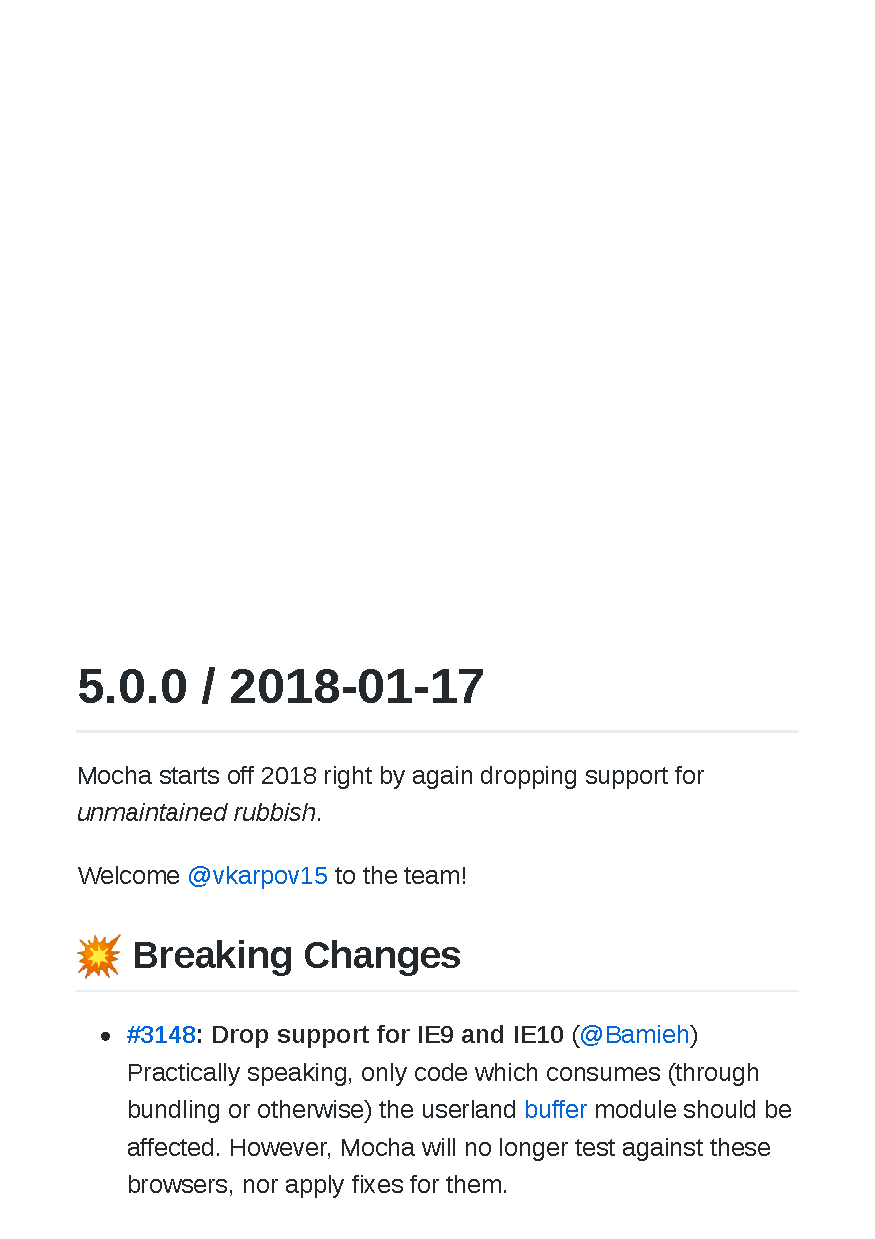
\includegraphics[scale=0.5]{figuras/bc_documentation_mocha.pdf}}\quad
        \subfigure[]{\label{fig:bc_documentation_other} 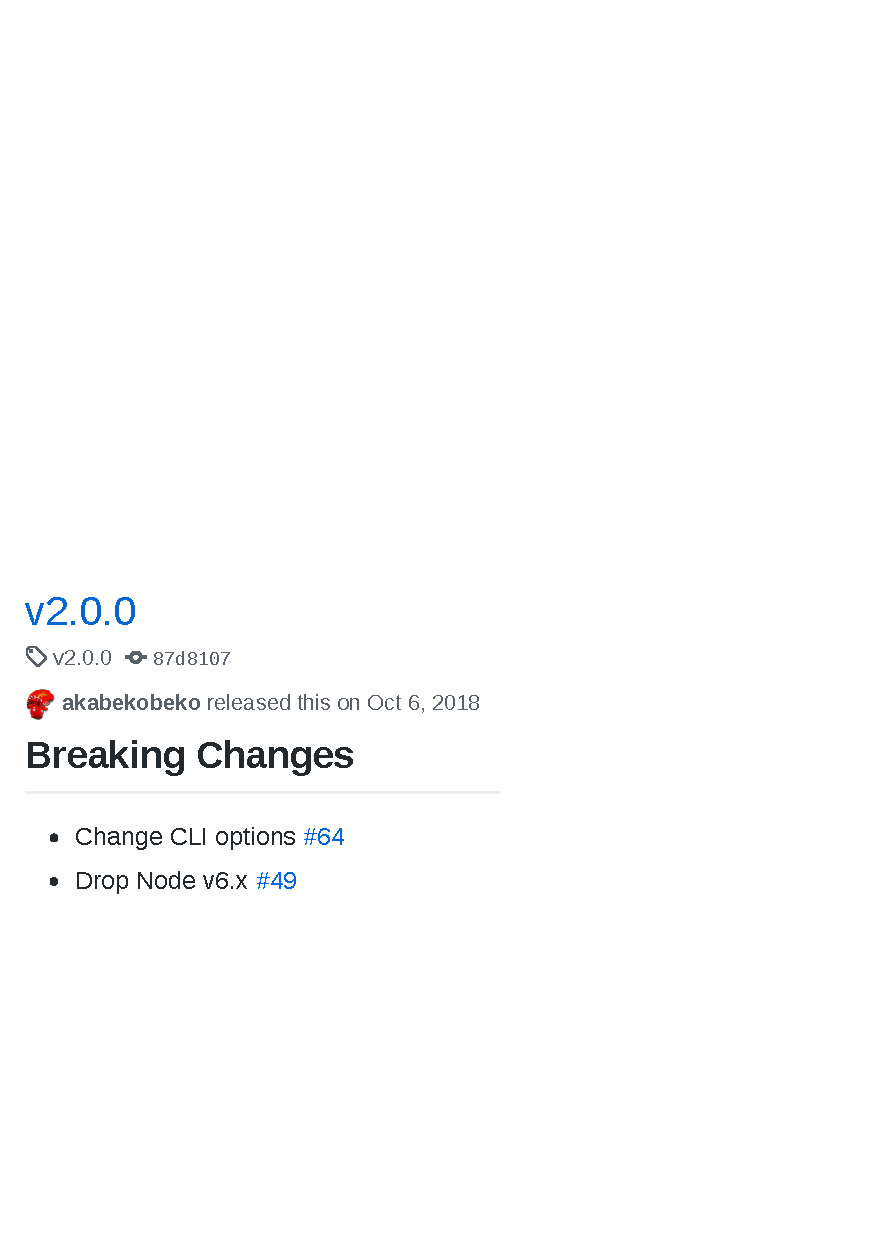
\includegraphics[scale=0.5]{figuras/bc_documentation_other.pdf}}
    }
    \caption{Exemplo de \textit{break changes} documentadas em \textit{changelogs} e \textit{relese-notes}}
    \label{fig:result_rq1_once_twice_three}
\end{figure}

Também foi buscado em \textit{issues} e \textit{pull-requests} por comentários indicando as causas das \textit{breaking changes}. Após descobrir as alterações que introduziram as \textit{breaking changes}, foram analisadas e agrupadas cada uma dessas alterações em categorias mais genéricas possíveis. Por exemplo, todas as alterações relacionadas com mudança no tipo de variáveis foram agrupadas em uma categoria chamada \textit{Alteração de tipo de objeto}. Também foi analisado o nível do Versionamento Semântico que a \textit{breaking change} foi introduzida pelo provedor e consertada pelo provedor ou cliente, bem como o local onde as \textit{breaking changes} foram documentadas (\textit{issues/pull-requests/changelogs}).

%---------------------------------------------------%
%----------------------RQ3--------------------------%
%---------------------------------------------------%

\section{QP3. Como os clientes se recuperam das \textit{breaking changes}?}
\label{sec:qp3}

\subsubsection{Motivação}
\label{sec:qp3:motivation}

Uma \textit{breaking change} pode impactar um pacote cliente através de uma atualização \textit{implícita} ou \textit{explícita} de seu pacote provedor. Uma atualização implícita ocorre quando o cliente especificou o seu provedor como um \textit{range} de versões no \textit{package.json}. Então o \textsf{npm} descarrega automaticamente a nova \textit{release} do provedor. Já uma atualização explícita ocorre quando o cliente atualiza manualmente a versão do provedor no \textit{package.json} e o \textsf{npm} descarrega a nova versão especificada pelo cliente. Após uma \textit{breaking change}, o cliente pode se recuperar realizando uma alteração no seu código, aguardando uma nova \textit{release} do provedor que venha a consertar a \textit{breaking change} ou o cliente pode realizar um \textit{downgrade/upgrade} na versão do provedor.

As \textit{breaking changes} podem ser introduzidas pelo provedor \textit{direto} ou pelo \textit{indireto}, uma vez que os clientes dependem de poucos provedores diretos mas dependem de muitos provedores indiretos \cite{npm-seven}. Mesmo quando o cliente tem poucos provedores diretos, muitos provedores indiretos podem propagar \textit{breaking changes}. Quando uma \textit{breaking change} se manifesta nos pacotes clientes, esses devem se recuperar uma vez que eles precisam executar sem erros e, também, eles podem ser provedores de outros pacotes nessa árvore de dependências. Portanto, uma \textit{breaking change} pode ser continuamente propagada enquanto não for consertada por nenhum dos pacotes. Até mesmo quando as \textit{breaking changes} podem ser consertadas atualizando para uma nova versão do provedor, os pacotes clientes precisam resolver manualmente as incompatibilidades que ainda existem \cite{Foo:2018:ESC:3236024.3275535}. Então, entender o comportamento da manifestação das \textit{breaking changes} pode ajudar os desenvolvedores a compreenderem quais são as maneiras mais efetivas e rápidas para se recuperar das \textit{breaking changes}.

\subsubsection{Método}
\label{sec:qp3:approach}
Todas as informações usadas para responder esta questão de pesquisa foram recuperadas dos repositórios dos pacotes clientes. Foi procurado nesses repositórios por informações sobre o erro e como os cliente se recuperaram da \textit{breaking change}. As seguintes informações foram analisadas:

\begin{itemize}
    \item \textbf{\textit{Commits:}} foi analisado manualmente os próximos \textit{commits} no repositório do cliente a partir da data da \textit{release} que contém a \textit{breaking change}. Foram analisados principalmente os \textit{commits} que alteraram o \textit{package.json} para verificar se o cliente realizou um \textit{downgrade/upgrade} ou se o cliente removeu ou substituiu o provedor.

    \item \textbf{\textit{Changelogs:}} o cliente pode mencionar nos \textit{changelogs} e nas \textit{release-notes} como foi realizada a recuperação da \textit{breaking change}, principalmente se o cliente realizou um \textit{downgrade/upgrade} na versão do provedor. Também, se o cliente consertou a \textit{breaking change} diretamente no seu código, provavelmente há essa informação nos \textit{changelogs}. Ao todo, 48\% dos repositórios dos clientes continham \textit{changelog} ou \textit{release-notes}.
    
    \item \textbf{\textit{Pull-requests/Issues:}} foi procurado por \textit{pull-requests} e \textit{issues} no repositório do cliente que deveria consertar, ou conter informações sobre a \textit{breaking change}. \textit{Pull-requests/issues} nomeadas como \textit{Update provider}, \textit{Fix provider errors}, \textit{Fix tests} indicavam a presença de alguma alteração que foi realizada devido às \textit{breaking changes}.
\end{itemize}

Para cada caso de \textit{breaking change} foi recuperado a árvore de dependências do cliente até o provedor que introduziu a \textit{breaking change}. Por exemplo, em nosso segundo exemplo motivacional (Capítulo \ref{cap:exemplos}) foi recuperado a árvore de dependências a partir do cliente até \textsf{broccoli-asset-rev$\rightarrow$broccoli-filter$\rightarrow$broccoli-plugin} (Figura \ref{fig:dependency_tree}). Com isso foi analisada a quantidade de \textit{breaking changes} introduzida por provedores diretos e indiretos. 

Também foi investigado os dados sobre quando a \textit{breaking change} foi introduzida, consertada, qual pacote consertou e como foi realizada a correção. Assim foi analisado o tempo que as \textit{breaking changes} levaram para serem consertadas e quais são as principais maneiras com que os clientes se recuperam das \textit{breaking changes}. Ainda foi analisado os casos onde o provedor consertou a \textit{breaking change} e, ainda assim, o cliente realizou um \textit{upgrade/downgrade} da versão do provedor. Por fim, foi verificado como a versão dos provedores foram alteradas pelos clientes e como a documentação da \textit{breaking change} influenciou na velocidade com que as \textit{breaking changes} foram consertadas.